\chapter{
Modeling Encounter Probability
%%%%Modeling Covariate Effects in SCR Models
}
\markboth{Encounter probability}{}
\label{chapt.covariates}

\vspace{.3in}

\begin{comment}
XXXXXXXXXXXXXXXXXXXXXXXXXXXX
XXXXXXXXXXXXXXXXXXXXXXXXXXXX
- check on section for ``see sec. gof.sec.XXXXX'' comment
XXXXXXXXXXXXXXXXXXXXXXXXXXXXXXXXXXXXX
XXXXXXXXXXXXXXXXXXXXXXXXXXXXXXXXXXXXXXXX
\end{comment}


\section{Introduction}

% In previous chapters we showed how to fit basic spatial
% capture-recapture models using Bayesian analysis (in {\bf WinBUGS} or
% {\bf JAGS};
% Chapt. \ref{chapt.scr0}) or by classical likelihood methods
% (Chapt. \ref{chapt.mle} or using \mbox{\tt secr}).  These basic models involved only constant
% parameter values that did not vary in response to covariates of any
% type.  However, in practice, investigators are invariably concerned
% with explicit factors or covariates that might influence variation in
% parameters. Traditionally, in the non-spatial capture recapture
% literature, such models were called ``model $M_t$'', ``model
% $M_h$'', or ``model $M_b$'', identifying models that account for
% variation in detection probability as a function of time, ``individual
% heterogeneity'' or ``behavior'', where behavior describes
% whether or not an individual had been previously captured.  In SCR
% models, more complex covariate models are possible because we might
% also have trap-specific covariates, or covariates that vary spatially
% over the landscape.

% So far, we have only covered 
% how to use only the basic model in various software packages and 
% the suite of possible encounter models
% (e.g., the Binomial, Poisson, and Multinomial encounter models) for
% dealing with different types of sampling.  However, we have not
% considered different detection functions or covariates that can affect
% the parameters of the detection function, including those that may
% arise from the individual or the trap device.
% Most detection functions include a baseline encounter
% rate termed $\lambda_0$ (or $g_0$ for the detection probability when
% we use a logit link for the detection function) and a shape parameter
% termed $\sigma$, which takes on different interpretations depending on
% the selected function.  Such covariates
% include time (e.g., day of year, or season), behavior (e.g., has the
% individual been previously captured), sex of the individual, and trap
% type (e.g., various camera types, or different constructions for hair
% snares).


In previous chapters we showed how to fit basic spatial
capture-recapture models using Bayesian analysis (in {\bf WinBUGS} or
{\bf JAGS};
Chapt. \ref{chapt.scr0}) or by classical likelihood methods
(Chapt. \ref{chapt.mle} or using \mbox{\tt secr}). We covered a suite of possible encounter models
(e.g., the Binomial, Poisson, and Multinomial) for
dealing with different types of sampling. We have not, however,
described a general framework for modeling covariates that might
influence encounter probability of individuals, traps or over time.
In practice, 
investigators are invariably concerned
with explicit factors or covariates that might influence variation in
parameters. Such covariates
include time (e.g., day of year, or season), behavior (e.g., is there an 
effect of trapping on subsequent capture probabilities), sex of the individual, and trap
type (e.g., various camera types, or different constructions for hair
snares). Traditionally, in the non-spatial capture recapture
literature, such models were called ``model $M_t$'', ``model
$M_h$'', or ``model $M_b$'', identifying models that account for
variation in detection probability as a function of time, ``individual
heterogeneity'' or ``behavior'', where behavior describes
whether or not an individual had been previously captured. In SCR
models, more complex covariate models are possible because we might
also have trap-specific covariates, or covariates that vary spatially
over the landscape, and because we generally have more than one 
parameter describing the detection function:
Most detection functions include a baseline encounter
rate ($\lambda_0$) or probability ($p_0$) parameter, and a shape parameter
($\sigma$), which takes on different interpretations depending on
the specific encounter probability function under consideration. 

In this chapter, we generalize the basic SCR model to accommodate both 
alternative detection functions as well as
many different kinds of covariates. We focus on the binomial encounter
model used throughout Chapts. \ref{chapt.scr0} and \ref{chapt.mle} and
the Gaussian encounter model (also called the ``half-normal'' model in
the distance sampling literature), 
but the extension to other encounter and detection models is
straightforward (and other distance functions are considered in sec. \ref{covs.sec.detfunc}). 
Specifically, we consider three distinct types of
covariates -- those which are fixed, partially observed or completely
unobserved (latent).  Fixed covariates are those that are fully
observed; for example, the date of all sampling occasions.  Partially
observed covariates are those which are not known for all
observations; for example, the sex of an individual cannot always be
determined from photos taken during camera trapping.  Even if we are
able to observe the sex of all individuals sampled, we cannot know it
for those individuals never observed during the study.  And finally,
unobserved covariates are those which we cannot observe at all, for
example, the home range size of individuals, or unstructured random
``individual effects''.


We will see that models containing these different types of
covariates are relatively easy to describe in {\bf WinBUGS} or
{\bf JAGS}, and
therefore to analyze using Bayesian analysis of the joint likelihood
based on data augmentation thus providing a coherent and flexible
framework for inference for all classes of SCR models.  Throughout the
chapter, we will continue to develop the analysis of the black bear
study introduced in Chapt. \ref{chapt.closed}, using the software
\jags.  We also
consider the likelihood analysis of many of these models; to do so, we
will demonstrate the use of the {\bf R} package \secr~ and how to do model
comparison with AIC (sec. \ref{likelihood.secr} at the end of the chapter).
There are other types of covariates that we do {\it not} cover in this
chapter; for example, covariates that vary across the
landscape might affect density, and we consider these covariates in
Chapt. \ref{chapt.state-space}.
Alternatively, these landscape covariates might affect the way individuals use
space. There are probably very few circumstances under which animals use all 
space uniformly and we develop more realistic models of encounter
probability in which covariates affect space usage in Chapt. \ref{chapt.ecoldist}.


\section{Encounter Probability Models}
\label{covs.sec.detfunc}

In Chapt. \ref{chapt.scr0}, we developed a basic spatial capture
recapture model using a standard distance function based on the kernel
of a normal (Gaussian) probability distribution:
\[
p_{ij} = p_{0} \exp(-\alpha_{1} *||{\bf x}_{j}-{\bf s}_{i}||^2)
\]
where $||{\bf x}_{j}-{\bf s}_{i}||$ is the distance between ${\bf
  x}_{j}$ and ${\bf s}_{i}$ and
$\alpha_{1} = 1/(2*\sigma^2)$.
We argued (see Sec. \ref{scr0.sec.implied}) that this model corresponds to
an explicit model of space usage -- namely, that individual locations
are draws from a bivariate normal distribution. We also mentioned that
other detection models are possible, including a logit model of the
form:
\begin{equation}
	\mbox{logit}(p_{ij}) = \alpha_{0} + \alpha_1 ||{\bf x}_{j}-{\bf s}_{i} ||.
\label{covariates.eq.logit}
\end{equation}
However, there's nothing preventing us from constructing a myriad of
other models for encounter probability as a function of distance.
The most
commonly used encounter probability models
 are also those used in the distance
sampling literature: the half-normal (Gaussian), the hazard, and the negative
exponential.  The negative exponential model is: 
\[
p_{ij} = p_{0}*\exp(-\alpha_{1} *||{\bf x}_{j}-{\bf s}_{i}||)
\]
where we define
$\alpha_{1} = 1/\sigma$.
We could use the general power model \citep{russell_etal:2012}: 
\[
p_{ij} = p_0*\exp(-\alpha_{1} *||{\bf x}_{j}-{\bf s}_{i}||^{\theta} )
\]
of which the
Gaussian and exponential models are special cases.  Another model that
could be considered is the Gaussian hazard rate model \citep{hayes_buckland:1983}:

\[
p_{ij} = 1-\exp(-\lambda_{0}* \exp(-\alpha_{1} *||{\bf x}_{j}-{\bf
  s}_{i}||^{2}) )
\]
which was previously discussed in Sec. \label{scr0.sec.binomial}.


In each of the cases, the relationship of $\alpha_1$ to $\sigma$ varies and must
be properly specified.  The {\bf R} package
{\tt secr} allows the user to access 12 different detection models, of which
some are only used for simulating data (see Table \ref{covariates.tab.detmodels}). These detection
functions can also be implemented in {\bf R}, {\bf WinBUGS},
{\bf JAGS} etc..


\begin{table}[ht]
\centering
\caption{
  Basic encounter probability models (``distance functions'')
 available in \mbox{\tt secr}.  (Table taken from
  the 
\mbox{\tt secr}
  help files). Notation deviates from that used in the text.
  In this table $g_{0}$ is the baseline encounter rate or probability
  parameter used in \secr~ but this is equivalent to our $p_{0}$ or
  $\lambda_{0}$ depending on context. $d$ is distance defined as we have done throughout,
  as the distance between the activity center and the trap.
  One can read more on this specific table by loading the \secr~ package and using the
  {\tt help} command in {\bf R} ({\tt ?detectfn}).
}
\begin{tabular}{cccl}
\hline \hline
 & Name & Params & Function  \\ \hline
 \\
0 & half-normal &$g_0$, $\sigma$          &  $g(d) = g_0 e^{-d^2 / (2  \sigma^2)}$  \\
1 &hazard rate  & $g_0$, $\sigma$, z      &  $g(d) = g_0 (1 - e^{-(d / \sigma) ^{-z} })$ \\
2 &exponential   &$g_0$, $\sigma$    &  $g(d) = g_0 e^{- d / \sigma}$ \\
3 &compound half-normal  & $g_0$, $\sigma$, z & $g(d) = g_0 [1 - \{1 - e^{-d^2 /(2 \sigma^2)}\}^z]$ \\
4 &uniform     & $g_0$, $\sigma$     &
\parbox[t]{2in}{ $g(d) = g_{0}, d \leq \sigma$; \\
                 $g(d)= 0$, otherwise
} \\
5 &w exponential            & $g_0$, $\sigma$, w &
\parbox[t]{2in}{ $g(d) = g_{0}, d < w$; \\
                 $g(d) = g_{0} e^{(- (d - w) / \sigma)}$, otherwise
} \\
6 &annular normal           & $g_0$, $\sigma$, w & $g(d) = g_0 e^{(-(d-w)^2 / (2 \sigma^2))}$ \\
7 &cumulative lognormal     & $g_0$, $\sigma$, z & $g(d) = g_0 [1 -F{(d-\mu)/s)}]$  \\
8 &cumulative gamma         & $g_0$, $\sigma$, z  & $g(d) = g_0 \{ 1 - G (d; k,  \theta) \}$  \\
9 &binary signal strength   & $b_0$, $b_1$       & $g(d) = 1 - F \{- (b_0 + b_1 d) \}$ \\
10&signal strength          & $\beta_0$, $\beta_1$,S  &
  $g(d) = 1 - F[ \{c - (\beta_0 + \beta_1 d)\} / S]$  \\
11&signal strength spherical&  $\beta_0$, $\beta_1$,S & 
\parbox[t]{2in}{ $g(d) = 1 - F[\{c - (\beta_0 + \beta_1(d-1)- 10 * log_{10} ( d^2 ) ) \} / S]$ 
} \\ \hline
%$g(d) = 1 - F[\{c - (\beta_0 + \beta_1 * (d-1)$ \\ 
%& & & $- 10 * log10 ( d^2 ) ) \} / sdS ]$ \\
\end{tabular}
\label{covariates.tab.detmodels}
\end{table}


Insofar as all these encounter probability models
are symmetric and stationary, they are pretty
crude descriptions of space usage by real animals. This is not to
say they are inadequate descriptions of the data and, as we discuss in
Chapts. \ref{chapt.rsf} and \ref{chapt.ecoldist}, we can use them as the
basis for producing more realistic models of space usage.  

By changing the encounter probability model
and the specification of
$\alpha_1$, we can basically create any distance function for the
data. It is important to note that $\sigma$ is not comparable under
these different encounter probability models
and should not be
regarded as ``home range radius'' in general.  While there is
generally a relationship between $\sigma$ and home range size, that
relationship varies depending on the model under consideration. We
demonstrate how to fit different encounter probability models
 in the Bayesian
framework here, and then provide a section on the likelihood analysis
(in \secr) in a separate section below.

\subsection{Bayesian Analysis with {\tt bear.JAGS}}

To demonstrate how to incorporate various types of covariates into
models for encounter probability using {\bf JAGS}, we return to the
data collected during the Fort Drum bear study.  This data set was first
introduced in Chapt. \ref{chapt.closed}, but, to refresh your memory,
there were 38 baited hair snares that were operated between June and
July 2006.  The snares were checked each week for a total for $K=8$
sample occasions and $n=47$ individual bears were encountered at least
once.  The data are provided in the {\bf R} package \mbox{\tt scrbook}
and an {\bf R} function called {\tt bear.JAGS} allows the user to
easily pick which model to analyze.  The function {\tt bear.JAGS} will
set up the data, write the model, define the MCMC specifications
(e.g., initial values, etc.) and, finally, run the selected model in
{\bf JAGS}. In addition to choosing which model to run, the user can
also specify the number of chains, iterations and length of the
burn-in phase. Calling the function will provide all the code to
implement the models independently as well.  In the following sections
we will present the model code and output for the most commonly
employed models; for all analyses we ran 3 chains with a burn-in of
500 iterations and 20000 saved iterations.

\subsection{Bayesian Analysis of encounter probability models}
% We start here by presenting the basic SCR model with no covariates and
% the half normal distance function.

In Panel \ref{covariates.panel.basicSCR}, we present the basic SCR
model and show how to specify the negative exponential encounter
probability model.
  To call each of these from the function {\tt bear.JAGS} set
{\tt model='SCR0'} or {\tt model='SCRexp'} in the function call,
respectively.  To reduce repetition of the R coding, we include the
basic code here and then only show modifications when necessary throughout
the chapter.  All of the R coding can be found within the {\tt bear.JAGS}
function as well.   To begin, the required R libraries are installed and 
then we attached the Ft. Drum bear dataset.  The bear dataset includes 
a 3-d data array (called \mbox{\tt bearArray} in our code), 
with dimensions $\mbox{\tt nind} \times \mbox{\tt ntraps} \times \mbox{\tt nreps}$ 
representing the capture histories of $\mbox{\tt nind}$ captured individuals at
$\mbox{\tt ntraps}$ trap locations.  In the Bayesian analysis, data augmentation is
used to estimate $N$ and therefore the \mbox{\tt bearArray} data must be augmented with
$M - \mbox{\tt nind}$ all zero encounter histories.  In models without time dependence,
the augmented \mbox{\tt bearArray} (called \mbox{\tt Yaug} in the code) will be reduced
to a 2 dimensional array (denoted \mbox{\tt y} in the code) that has dimensions 
 $\mbox{\tt M} \times \mbox{\tt ntraps}$.

\begin{verbatim}
>library(rjags)  #load the necessary libraries
>library(scrbook)

>data(beardata)   #attach the bear data for Ft. Drum
>ymat<-beardata$bearArray
>trapmat<-beardata$trapmat
>nind<-dim(beardata$bearArray)[1]
>K<-dim(beardata$bearArray)[3]
>ntraps<-dim(beardata$bearArray)[2]
>M=650
>nz<-M-nind

  #create augmented array
>Yaug <- array(0, dim=c(M,ntraps,K))
>Yaug[1:nind,,]<-ymat
>y<-apply(Yaug,1:2, sum)

\end{verbatim}


The function {\tt bear.JAGS} also establishes the upper 
and lower limits on the state space by centering the trap
array coordinates (which are imported with the {\tt beardata}
and saved in the code above as {\tt trapmat}) and then buffering by 20km.  


\begin{panel}[htp]
\centering
\rule[0.1in]{\textwidth}{.03in}
{\small
\begin{verbatim}
model{
alpha0 ~ dnorm(0,.1)                         # Prior distributions
logit(p0)<- alpha0
alpha1<-1/(2*sigma*sigma)
sigma ~ dunif(0, 15)
psi ~ dunif(0,1)

for(i in 1:M){
 z[i] ~ dbern(psi)
 s[i,1] ~ dunif(xlim[1],xlim[2])
 s[i,2] ~ dunif(ylim[1],ylim[2])
for(j in 1:J){
  d[i,j]<- pow(pow(s[i,1]-X[j,1],2) + pow(s[i,2]-X[j,2],2),0.5)
  y[i,j] ~ dbin(p[i,j],K)
  p[i,j]<- z[i]*p0*exp(- alpha1*d[i,j]*d[i,j])  # Gaussian model
 #p[i,j]<- z[i]*p0*exp(- alpha1*d[i,j])         # exponential model
 }
}
N<-sum(z[])
D<-N/area
}
\end{verbatim}
}

\rule[-0.1in]{\textwidth}{.03in}
\caption{
\jags~ model specification for a basic SCR model with Gaussian
distance 
function and the alternative exponential distance function.}
\label{covariates.panel.basicSCR}
\end{panel}

Applying the SCR model with Gaussian encounter probability model
 provides an
estimate (posterior mean) of $D = 0.167$ bears per $km^2$ and with the
negative exponential encounter probability model
the posterior mean  is virtually the
same $D = 0.167$.  In distance sampling, the use of different
encounter probability models
 often results in very different estimates of density
(especially when using the negative exponential model).  There are
two main reasons why the different models  may have less of
an impact on the density estimates under the SCR models.  First, we
can estimate the baseline encounter probability
 parameter ($p_0$).  
%%%
%%% BETH: I feel like the point (or maybe both points) made below 
%%% are not extremely clear. Is it possible to clarify this point a little?
%%% I agree it needs to be said but it seems a bit vague-ish now
In most
distance sampling models, detection at distance 0 is set to 1.  In
Table \ref{covariates.tab.SCR0exp}, the posterior mean of $p_0$ is
0.11 under the Gaussian  model and 0.34 under the negative
exponential model.  The larger baseline encounter probability
 under the negative
exponential model reduces the impact of the having ``no shoulder".
Secondly, the distance function here is governing 'movement' of
individuals (which we have more information on than in distance
sampling), not the whole detection process, so the shape of the
distance function does not impact the density estimation as much.

In all analyses it is important to check that the size of the
augmented data set ($M$) is sufficiently large and does not impact 
the estimate of $N$.  Here, the 97.5\%
percentile for $N$ is 628 (Table \ref{covariates.tab.SCR0exp}), thus not reaching our $M=650$ value.
We could also increase
$M$ and compare the posterior of $N$ under the different scenarios as another check 
that the data augmentation is sufficient.  

\begin{table}[ht]
\centering
\caption{Posterior summaries of SCR model parameters having 
  different encounter probability models, for the Fort Drum black bear data.}
\begin{tabular}{crrrr}
\hline \hline
Parameter & Mean & SD & 2.5 & 97.5 \\
\hline

Gaussian  &   &      &           &        \\
\hline
$D$    &   0.17   & 0.022     &  0.122 & 0.207  \\
$N$    &  500.63 & 66.652  & 371.000   & 628.000       \\
$p_0$  &    0.11  & 0.014   & 0.081& 0.135     \\
$\psi$  &   0.77  & 0.104    & 0.566 & 0.966    \\
$\sigma$ &  1.99 & 0.131  &1.762 & 2.275     \\

Exponential &   &      &          &        \\
\hline
$D$  &   0.17 &  0.022 &	0.130		& 	0.210	 \\
$N$   &  512.06 &  65.771  &	382.000		& 	634.000	 \\
$p_0$  &    0.34 &   0.056  &	0.246	& 0.465		 \\
$\psi$  &   0.79  &  0.102  &	0.584		& 	0.974	 \\
$\sigma$ &  1.12  & 0.095  &	0.951		& 	1.323	 \\ \hline
\end{tabular}
\label{covariates.tab.SCR0exp}
\end{table}

A very important consideration when using different distance functions is the
interpretation of $\sigma$.  The estimate of $\sigma$ under the negative exponential model is
$1.12$, which is distinct from our
estimate of $\sigma$ under the Gaussian model, $\sigma = 1.996$.
The interpretation
of $\sigma$ in the two models is really quite distinct. In the normal
model it can be interpreted as the standard deviation of a bivariate
normal movement model whereas the manner in which $\sigma$ relates to
``area used'' for the negative exponential model has nothing to do
with a bivariate normal model of movement.  This highlights that it is
important for the user to know what distance function is used and what
the interpretation of $\sigma$ might be in relation to the home range size.
This relationship was discussed in Sec. \ref{scr0.sec.implied}.

We  now move onto incorporating
covariates into the model using the {\bf JAGS}
language.  For this part, we will stick with the Gaussian encounter
probability model
 shown in the Panel \ref{covariates.panel.basicSCR} above.
%%%


\section{Modeling Covariate Effects}

The basic strategy for modeling covariate effects is to include them
on the baseline encounter rate or probability parameter, $p_{0}$ (or
$\lambda_{0}$), or the scale parameter of the encounter model,
$\sigma$, or in some cases, both parameters.

Broadly speaking, we recognize (here) 3 types of covariates. Fixed
covariates that are fully observable and might vary by trap alone
(e.g., type of trap, baited or not, disturbance regime, even habitat),
sample occasion (e.g., day of season or weather conditions), or both
(e.g., behavior, weather - if over a large region).  Another class
of covariates are those which vary at the level of the individual (and
possibly also over time).  As a technical matter, and as noted before,
these are different from fixed covariates because we cannot see all of
the individuals and the covariates are almost always incompletely
observed (if at all).  The lone exception is the behavioral response
to capture which is known for all individuals, captured or not (an
animal never captured/observed has never been captured before).  We
noted may times before that space itself (i.e., the activity centers)
is a type of individual covariate and this notion actually helped us
derive the fully spatial capture-recapture model from the traditional,
non-spatial model (Chapt. \ref{chapt.closed}). We do not get to observe
the activity center for any individuals, but for individuals that are
encountered we get to observe some information about it in the form of
which traps the individual was encountered in.  And finally, we have
completely unobserved covariates such as heterogeneity in home range
size.  We consider heterogeneity in a separate section below since 
alone there are 
a suite of models for describing  latent heterogeneity. 

\begin{table}[ht]
\centering
\caption{Examples of different types of covariates in SCR models.}
\begin{tabular}{cr}
\hline \hline
Covariate type & Examples \\
\hline
individual & sex, age, home range \\
trap  &  baited/not, habitat (see also Chapter \ref{chapt.rsf}) \\
time  &  season, shedding,  weather  \\
individual x time    &    global behavioral response \\
trap x time     &       trap failures  \\ 
individual x trap x time  &   local behavioral response  \\ \hline
\end{tabular}
\label{covariates.tab.covclass}
\end{table}


To develop covariate models, we assume a standard sampling design in which an
array of $J$ traps is operated for $K$ sample occasions, which produces
encounter histories for $n$ individuals.  For the null model, there
are no time-varying covariates that influence encounter, there are no
explicit individual-specific covariates, and there are no covariates
that influence density.  For fixed effects, those which we observe
fully, we can easily incorporate these into the encounter probability
model, just as we would do in any standard GLM or GLMM, on some
suitable scale for the encounter probability, $p_{ijk}$. For example,
\begin{eqnarray*}
\mbox{logit}(p_{0,ijk}) &=& \alpha_0 + \alpha_2*C_{ijk} \\
p_{ijk} &=& p_{0,ijk} \exp(- \alpha_1*||{\bf x}_{j}-{\bf s}_{i}||^2) 
\end{eqnarray*}
where $C_{ijk}$ is some covariate that varies (potentially) by
individual ($i$), trap ($j$) and occasions ($k$), and
$\alpha_2$ is the coefficient to be estimated.
 How we define specific covariates (e.g., trap specific
versus individual specific) will influence exactly how we include them
in the model. Table \ref{covariates.tab.covclass} shows examples of covariates by
type -- trap, individual, and time -- and also gives examples of some combined types.
These are the types of covariates we will specifically address in this chapter demonstrating
how to analyze the different
 types in the following sections.  
%For example, $C$ might vary by
%individual, trap, sampling occasion or combinations of these.

\subsection{Date and Time}

Often, researchers are interested in modeling the effect of date or
chronological time on 
encounter probability. For example, in a long term hair snare study,
we may expect that seasonal shedding \citep{wegan_etal:2012} will
influence encounter probabilities directly. Or, we may expect
behaviors such as denning, mating, etc., to influence the encounter of
certain species at certain times of year \citep{kery_etal:2011}.
There are two common ways to incorporate date or time information into
a model for encounter probability. For cases with a small number of
sampling occasions we can fit a time-specific intercept (analogous to
``model $M_{t}$'' in classical capture-recapture
\citep{otis_etal:1978}). In this model, there are $K$ sampling
occasion-specific parameters to reflect potential variation in
sampling effort or other factors that might vary across samples.
Alternatively, we can model parametric functions of date or time such
as polynomial or sinusoidal functions.

In the first case, we allow each sampling occasion, $k$, to have its
own baseline encounter probability, e.g.,
\[
\mbox{logit}(p_{0,k}) = \alpha_{0,k}
\]
so that
\[
p_{ijk} = p_{0,k} \exp(- \alpha_1*||{\bf x}_{j}-{\bf s}_{i}||^2).
\]
This description of the model includes $k$ occasion-specific baseline
encounter probabilities.  Thus, if there were 4 sampling occasions, then
there are 4 different baseline encounter probabilities.  We imagine
that complete time-specificity of $p_{0}$ 
(i.e., one distinct value for each sample occasion)
would be most useful in situations
where there are just a few sampling occasions (if there are many, this
formulation will dramatically increase the number of parameters to be
estimated) or we do not expect systematic patterns over time (e.g.,
explainable by a polynomial function).

To implement this in \jags, $\alpha_0$ has to be
estimated for each time period $k$ either using an index vector or
dummy variables (as described in Chapt. \ref{chapt.modeling} and Sec. 
\ref{closed.sec.timebehavefx})and this can be done by only 
changing only a few lines in Panel \ref{covariates.panel.basicSCR}.

\begin{verbatim}
alpha0[k] ~ dnorm(0,.1)
logit(p0[k])<- alpha0[k]
.......
.......
y[i,j,k] ~ dbin(p[i,j,k],K)
p[i,j,k]<- z[i]*p0[k]*exp(- alpha1*d[i,j]*d[i,j])
\end{verbatim}

Since the model contains a parameter for each time period, the
encounter histories must be time-dependent.  Thus, a 3-d data array
(called \mbox{\tt bearArray} in our code), with dimensions $\mbox{\tt
  nind} \times \mbox{\tt ntraps} \times \mbox{\tt nreps}$ is
required (recall that we use the 3-d augmented array called {\tt Yaug}
with dimensions $\mbox{\tt M} \times \mbox{\tt ntraps} \times \mbox{\tt nreps}$
for the Bayesian analysis). In addition to using the 3-d data array, the initial values
must be updated so that there are $K$ values generated for $\alpha_0$.
And finally, this means that another nested for loop is needed
in the code to account for the $K$ sample occasions.  A side note: the
computation time will increase quite a bit (this model for the bear
data may take up to 15 hours or more on your machine to obtain a
sufficient posterior sample).

Running this model with the function {\tt bear.JAGS} by setting {\tt
  model=SCRt}, returns estimates of density similar to those from the model 
  without covariates (see Table \ref{covariates.tab.SCRt}), but
now we have a characterization of variation in encounter probability
over time.  Encounter probability seems to increase for the first few
time periods before stabilizing around $0.14$, dropping off again at
the end of the study.  The differences in encounter probability from
the first time periods to the others might actually be due to
something like a behavioral response (see below) or possibly seasonal
differences in the efficiency of the sampling technique.  Researchers
have found that hair snares are more effective at different times of
the year (even within season) due to shedding
\citep{wegan_etal:2012}.  In this particular example, our density
estimates are similar to the base model, likely because the
differences in encounter probability
 between occasion were not that large.  In a
longer term study or in one with greater variation in the encounter
probability, the implication of such differences might have a bigger
impact on the estimates of density and $\sigma$.

\begin{table}[ht]
\centering
\caption{Posterior summaries of parameter estimates from a SCR model with time-dependent baseline 
encounter probability
 for the Ft. Drum black bear data set.}
\begin{tabular}{crrrr}
\hline \hline
Parameter & Mean & SD & 2.5 & 97.5 \\
\hline
$D$           &    0.17     &  0.02    & 0.13 & 0.21 \\
$N$           &   509.24 &  66.13  & 381  & 632  \\
$p_0 (t=1)$  &    0.06     & 0.02     & 0.03  & 0.10  \\
$p_0 (t=2)$  &    0.05  & 0.02  &      0.02 & 0.09  \\
$p_0 (t=3)$  &    0.15 &  0.03  &     0.09 & 0.22  \\
$p_0 (t=4)$  &    0.14 &  0.03  &     0.09 & 0.21  \\
$p_0 (t=5)$  &    0.15 &  0.03  &    0.09 &  0.22  \\
$p_0 (t=6)$  &    0.12 &  0.03  &    0.07 & 0.19  \\
$p_0 (t=7)$  &    0.15 &  0.03  &    0.09 & 0.22  \\
$p_0 (t=8)$  &    0.08 &  0.02  &    0.04 & 0.13  \\
$\psi$  &   0.78 &  0.10  &  0.58 & 0.97  \\
$\sigma$ & 1.96 &  0.12  &   1.73 & 2.22  \\ \hline
\end{tabular}
\label{covariates.tab.SCRt}
\end{table}

The 
occasion specific intercepts (basline encounter probability) model might not be the most
appropriate for all scenarios (and could require the estimation of
many parameters if we had many sampling occasions, take the wolverine
example from Chapt. \ref{scr0.sec.wolverine} where there were 165
daily sampling occasions).  Particularly in such a case, variation in
the encounter process over time is to be expected. For
example, if a camera trap study is conducted for an entire year, it is
expected that there would be behavioral patterns in individuals due to 
mating or denning. Instead of fitting a model with $K$ baseline
encounter probabilities, we can include date as a linear (or
quadratic, \ldots) effect. An example can be found in
\citet{kery_etal:2011} who incorporated a day-of-year covariate, both
as a linear and a quadratic effect, into their SCR model of European
wildcats; the data had been collected over a year-long period and cat
behavior was expected to vary seasonally thus influencing the
probability of encounter.  In these cases, we would specifically
incorporate day of year (variable ``\mbox{\tt Date}'') as a numeric
covariate as:
\begin{eqnarray*}
\mbox{logit}(p_{0,ijk}) &=& \alpha_0 + \alpha_2*\mbox{\tt Date}_{k} \\
p_{ijk} &= &p_{0, ijk} \exp(- \alpha_1*||{\bf x}_{j}-{\bf s}_{i}||^2)
\end{eqnarray*}
or a quadratic effect of day-of-year:
\begin{eqnarray*}
\mbox{logit}(p_{0,ijk})& =& \alpha_0 + \alpha_2*\mbox{\tt Date}_{k}
 + \alpha_3*\mbox{\tt Date}_{k}^{2} \\
p_{ijk} &= &p_{0,ijk} \exp(- \alpha_{1}*||{\bf x}_{j}-{\bf s}_{i}||^2)
\end{eqnarray*}
where the variable $\mbox{\tt Date}$ is an integer coding of
day-of-year, indexed to some arbitrary start point in time.



\subsection{Trap-specific covariates}

In some studies it makes sense to model encounter probability as a
function of local or trap-specific covariates. These can be one of two
types: genuine trap covariates that describe the trap or encounter site,
such as whether a trap is baited or not, or how many traps were set at a sampling location,
or what kind of bait was used, etc., or local covariates that
describe the likelihood that an animal would use the habitat in the
vicinity of the trap (see Chapt. \ref{chapt.rsf} for more on this situation).
We imagine that these covariates, of either type, should affect
baseline encounter probability.
%There are a variety reasons that traps may have a different baseline
%detection probability including if the trap is baited or not, if trap
%type varies (e.g., different camera models are used in a camera
%trapping study), or because of the habitat type (e.g., if the trap is
%located on a road/trail).  
For example, \citet{sollmann_etal:2011}
found a large difference in the encounter probability of jaguars due to traps
being located on roads, which the animals were using to travel along, as
opposed to traps placed off of roads.  In this case, the trap
type is a binary variable -- on/off road,
(another binary variable could be baited/non-baited).  We can write
this 
as:
\begin{eqnarray*}
\mbox{logit}(p_{0,j}) &= &\alpha_{0,type_j}  \\
p_{ijk}  & = & p_{0,j} \exp(- \alpha_1*||{\bf x}_{j}-{\bf s}_{i}||^2).
\end{eqnarray*}
Here, we use an index variable, ``type'', an integer 
value for the trap-specific covariate. 
Thus for our example of on/off
road, we would have $type_j = 1$ if trap $j$ is on a road and $type_j =
2$ otherwise, and we would estimate two separate $\alpha_{0}$
parameters -- one for
on-road and one for off-road cameras.  This general set up also allows
for more than 2 categories, say if  4 different camera models were
used in a study, we would use a set of 3 binary dummy variables to
allow for
estimation of the different encounter rates (i.e., the intercept). 
To express the model in terms of dummy variables using 
the 2-category example above, we would
specify our ``type'' vector as $\mbox{\tt Type}_j = 0$ if trap $j$ is on a road and
$\mbox{\tt Type}_j = 1$ otherwise, and write our model as
\[
\mbox{logit}(p_{0,ijk}) = \alpha_{0} + \alpha_{2} * \mbox{\tt Type}_{j}
\]
Now, $\alpha_{0}$ is the baseline encounter probability (on the logit
scale) for traps on a road ($\mbox{\tt Type}_j = 0$) and $\alpha_{2}$ is the effect on
baseline encounter probability 
of a trap being of $\mbox{\tt Type} = 1$. While these models are
equivalent, and should
yield identical results, sometimes one parameterization might work
better than the other in {\bf WinBUGS} or {\bf JAGS}
\citep{kery:2010}.

\subsection{Behavior or Trap Response by Individual}
\label{covariates.sec.behavior}

One of the most basic of encounter models is that which accommodates a
change in encounter probability as a result of initial encounter.
This is colloquially referred to as ``trap happiness'' or ``trap shyness'', or in other words, a
behavioral response of individuals to being captured \citep{otis_etal:1978}.
If a trap is baited
with a food source, an individual might come back for
more. On the other hand, if being captured is traumatic then an
individual might learn to avoid traps. Both of these types of
responses can occur in most species depending on the type of encounter
mechanisms being employed. Moreover, behavioral response can be either
global \citep{gardner_etal:2010jwm} or local  \citep{royle_etal:2011jwm}.
The local response is a trap-specific response 
%which likely makes more sense in most spatial situations. 
while a global response suggests that initial capture provides a net
increase or decrease in subsequent probabilities of capture (across
all traps). A behavioral response does not need to be enduring (i.e., persist
for the entire study after the individual has been captured/observed
for the first time) but can also be ephemeral, if, for example, an
animal only avoids a trap on the occasion immediately after it was
captured \citep{yang_chao:2005, royle:2008}. While we will focus the
examples in this chapter on enduring behavioral effects, extending
such a model to the case of an ephemeral response should not pose any
difficulties.

To describe these behavioral models we need to create a binary matrix that indicates
if an individual has been captured previously.  For the global
behavioral response, define the $n \times K$ matrix,
${\bf C}$, where $C_{ik} =1$
if individual $i$ was captured at least once prior to session
$k$, otherwise $C_{ik} = 0$.
\begin{eqnarray*}
\mbox{logit}(p_{0,ik})& =& \alpha_{0} + \alpha_{2}*C_{ik} \\
p_{ijk} &= &p_{0,ik} \exp(- \alpha_{1}*||{\bf x}_{j}-{\bf s}_{i}||^2)
\end{eqnarray*}
For the local behavioral response, which is trap specific, we create
an array, $C_{ijk}$, that indicates if an individual $i$ has been
previously captured in trap $j$ at time $k$.  We then include this in
the model in the exact same form as above (with the sole difference that both $C$ and $p$ 
are now also indexed by $k$):
\begin{eqnarray*}
\mbox{logit}(p_{0,ijk}) &= &\alpha_{0} + \alpha_{2}*C_{i,j,k} \\
          p_{ijk} &= &  p_{0,ijk} \exp(- \alpha_{1}*||{\bf x}_{j}-{\bf s}_{i}||^2)
\end{eqnarray*}

Since the behavioral response is occasion specific, to implement either the local or global 
response model in \jags~, we will have to use the 3-d array of the augmented
capture histories ($\mbox{\tt M} \times \mbox{\tt ntraps} \times
\mbox{\tt nreps}$) as we did for the time-varying encounter probability
model above. The code must loop over each sampling occasion, but otherwise, the model
varies only a little from the basic SCR model shown in Panel \ref{covariates.panel.basicSCR}.  
Here is the specification of the the occasion specific ($k$) loop:

{\small
\begin{verbatim}
for(k in 1:K){
  logit(p0[i,j,k])<- alpha0 + alpha2*C[i,j,k]
  y[i,j,k] ~ dbin(p[i,j,k],1)
  p[i,j,k]<- z[i]*p0[i,j,k]*exp(- alpha1*d[i,j]*d[i,j])
}
\end{verbatim}
}

Despite the minor changes to the {\bf BUGS} code, this model can require quite a 
bit of time and computational 
effort to carry out the behavior response models.  Implementing the behavioral 
models with the function {\tt bear.JAGS} by setting {\tt
model=SCRb or model=SCRB} for the local or global model respectively, 
returns the results, shown in Table \ref{covariates.tab.SCRb}.  
There is a strong
global behavior response suggested by the posterior mean of $\alpha_2 = 0.90$.  
The estimate of $N$ and subsequently $D$ are larger 
than under the model wihout a behavioral response, here we estimate $N = 577.56$ and in 
the SCR0 model, we estimated $N = 500$. 
This makes sense given the large estimate of $\alpha_2$, which suggests that bears
are trap happy.  In situations where animals are trap happy, 
the model tends to over estimate encounter probability
 (i.e., the bears that are 
never observed have a lower encounter 
probability than those that 
have been captured in the study) and thereby reduce the 
estimate of $N$.  We do not include the results here, but 
the estimates were similar under the local behavioral response
model.  

\begin{table}[ht]
\centering
\caption{Posterior summaries of parameter estimates from the SCR model with a 
global behavioral response of encounter for the Fort Drum black bear data set.}
\begin{tabular}{crrrr}
\hline \hline
Parameter & Mean & SD & 2.5\% & 97.5\% \\
\hline
$D$           &    0.19     &  0.02    & 0.15 & 0.21 \\
$N$           &   577.56 &  54.30  & 452  & 648  \\
$\alpha_0$  &    -2.81     & 0.24    & -2.91  & -2.36  \\
$\alpha_2$  & 0.90  &  0.23   & 0.45  &  1.35 \\
$\psi$  &   0.88 &  0.08  &  0.69 & 0.99  \\
$\sigma$ & 2.00 &  0.13  &   1.77 & 2.28  \\ \hline
\end{tabular}
\label{covariates.tab.SCRb}
\end{table}


\subsection{Individual Covariates}
\label{covariates.sec.sex}


Individual covariates are those which are measured (or measurable) on
individuals, so we get to observed them only for the captured
individuals. Sex is a simple example of an individual covariate, but
one of the most commonly used in capture-recapture studies. 
% It can be the
% case that it is missing for some captured individuals because
% frequently, in practice, we only imperfectly determine gender of many
% species.  
The sex of an individual can influence many aspects of its ecology and
behavior, including, for example, its home range size, frequency of
movement, and seasonal behavior. This is common in studies of
carnivores where females often have smaller home ranges than males
\citep{gardner_etal:2010jwm, sollmann_etal:2011}. Additionally, we may
find differences in the baseline encounter probability
 between males and females
because females may move around less frequently, or possibly because
they are less likely to use landscape structures that researchers may
target with sampling devices in order to increase sample size, such as
roads \citep[e.g.][]{salom-perez_etal:2007}.
Therefore, 
we can imagine that sex may impact both the baseline encounter
probability $\alpha_{0}$ and the typical home range
size, so that
$\alpha_{1}$ might also be sex-specific also.  The fully sex-specific model is:
\begin{eqnarray*}
\mbox{logit}(p_{0,i}) &= &\alpha_{0,sex_{i}}  \\
p_{ijk} &= &p_{0,i} \exp(- \alpha_{1, sex_{i}}*||{\bf x}_{j}-{\bf s}_{i}||^2)
\end{eqnarray*}
where $sex_{i}$ is a vector indicating the sex of
each individual (1 = male, 2 = female).  While we might know the sex of all
individuals observed in the study, we will never know the
sex of individuals that are not observed,
resulting in missing values \citep{gardner_etal:2010jwm}.
It is also possible that we may not be able to determine the sex of
individuals that are observed during the study. For example photographic
captures do not necessary result in pictures that allow the sex to be absolutely
determined, thus sometimes resulting in missing values of this covariate for animals
captured in the study.   We deal with this slightly differently
depending on the inference framework 
that we adopt (Bayesian or likelihood).  Here we demonstrate the Bayesian implementation 
and we discuss the likelihood approach using \secr~ in detail
below in Sec. \ref{covariates.secr.sex}.
Before proceeding with that, we note that it would be possible also to
model covariates directly on the parameter $\sigma$ (or its
logarithm), e.g., $\log(\sigma_{i}) = \theta_{1} + \theta_{2}
\mbox{\tt sex}_{i}$ (see Sec. \ref{gof.sec.aic}). 
One or the other (or perhaps {\it some} other)
parameterization may yield a better performing MCMC algorithm or provide a
more natural or preferred interpretation.
In the context of Bayesian analysis, given that priors are not
invariant to transformation of the parameters, this may be a
consideration in choosing the particular parameterization.


Specifying a fully sex-specific model for {\bf JAGS} is similar to the
time-specific model shown above. We need to use an index or dummy
variable to let $\alpha_0$ and/or $\alpha_1$ be defined separately for
males and females. The main difference in this sppecification is that we do
not observe sex for the augmented individuals. Therefore, we have
missing observations of the covariate for those individuals. As a
result, sex is regarded as a random variable and so the missing values
can be estimated along with the other structural parameters of the
model.    

Because we are regarding sex as a random variable, 
we have to specify a distribution for it.  
With only two possible outcomes, it is natural to suppose that
$\mbox{\tt Sex}_{i} \sim
\mbox{Bernoulli}(\psi_{sex})$ where the parameter $\psi_{sex}$ is the sex ratio of the
population.  
We assume our default non-informative prior for this parameter:
$\psi_{sex} \sim \mbox{Uniform}(0,1)$.  The model
specification in Panel \ref{covariates.panel.SCRsex} demonstrates how
to incorporate a partially observed covariate (i.e., ``sex'').
It is important to note that in the previous equation,
$sex_{i}$ is a vector with two categories indicating the sex of
each individual (e.g., 1 = male, 2 = female).  This corresponds
directly to having a binary indicator of sex 
(e.g., $\mbox{\tt Sex}_{i} = 1$ if individual $i$ is female, and 0 otherwise).
In the Bayesian formulation of the model, we use 
both the binary indicator ({\tt Sex}) and a categorical
indicator ($\mbox{\tt Sex2} = \mbox{\tt Sex} + 1$).  The former (termed {\tt Sex} in 
Panel \ref{covariates.panel.SCRsex}) allows us to specify the \mbox{Bernoulli} 
distribution for the random variable, and the latter (termed {\tt Sex2}) allows
us to use the dummy or indicator variable specification in the model.


In both {\bf JAGS} or {\bf BUGS} missing data are indicated by  {\tt
  NA} in the data objects passed to the program through the \mbox{\tt
  bugs} or \mbox{\tt jags} functions in {\bf R}. To set up the data,
we need to create a 
vector of length $M$ with the first $n$ elements being 0 if individual
$i$ is a female, or 1 if $i$ is a male (for the Fort Drum black bear
data the function {\tt bear.JAGS} extracts this information
automatically from the {\tt beardata} object), and the subsequent
$M-n$ elements being {\tt NA}.  It is generally a good idea to provide
starting values for the missing data, but we cannot provide starting
values for observed data; in this case where one vector (or other
object) contains both observed and missing data, initial values for
the observed data have to be specified as {\tt NA}.  The code snippet
below shows you how to set up the data including the {\tt Sex} vector
and the initial values function(the remainder of the code is identical to what we've
shown before).  

{\small
\begin{verbatim}
>sex<-beardata$sex  #the sex data for captured individual
>Sex<-c(sex-1, rep(NA, nz)) #sex enters as 1/2, this recodes it to 0/1
                            #so we can use Bernoulli distribution 

>data<-list(y=y,Sex=Sex, M=M,K=K, J=ntraps, xlim=xlim, ylim=ylim,area=areaX)
>params<-c('psi','p0','N', 'D', 'sigma', 'psi.sex')
>inits =  function() { list(z=c(rep(1,nind), rbinom(nz,1,0.5)),psi=runif(1), 
           s=cbind(runif(M, xlim[1],xlim[2]), runif(M,ylim[1],ylim[2])),
           psi.sex=runif(1),Sex=c(rep(NA, nind), rbinom(nz,1,0.5)), 
           sigma=runif(2,2,3),alpha0=runif(2)) }
\end{verbatim}
}
{\flushleft The} {\bf BUGS} model specification is shown in Panel 
\ref{covariates.panel.sexSCR}.

%%% BETH: NOTE: in this panel below I made a lot of notational changes
%%%  We need to catch these in the R package LATER this summer
 
\begin{panel}[htp]
\centering
\rule[0.1in]{\textwidth}{.03in}
{\small
\begin{verbatim}
model {

psi~dunif(0,1)                            # Prior distributions
psi.sex~dunif(0,1)
for(t in 1:2){                             
  alpha0[t]~dnorm(0,.1)
  logit(p0[t])<- alpha0[t]
  alpha1[t]<-1/(2*sigma[t]*sigma[t])
  sigma[t]~dunif(0, 15)
}

for(i in 1:M){
 z[i] ~ dbern(psi)
 Sex[i]~dbern(psi.sex)                    # Sex is binary
Sex2[i]<-Sex[i] + 1                       # Convert to categorical
 s[i,1]~dunif(xlim[1],xlim[2])
 s[i,2]~dunif(ylim[1],ylim[2])

for(j in 1:J){
d[i,j]<- pow(pow(s[i,1]-X[j,1],2) + pow(s[i,2]-X[j,2],2),0.5)
y[i,j] ~ dbin(p[i,j],K)
p[i,j]<- z[i]*p0[Sex2[i]]*exp(-alpha1[Sex2[i]]*d[i,j]*d[i,j])
}
}
N<-sum(z[])
D<-N/area
}
\end{verbatim}
}

\rule[-0.1in]{\textwidth}{.03in}
\caption{
\jags~ model specification for an SCR model with sex specific 
encounter probability parameters.}
\label{covariates.panel.SCRsex}
\end{panel}

Our estimate of density under the fully sex-specific model is still
very similar to the previous models (Table
\ref{covariates.tab.SCRsex}), and while the baseline detection was not
very different between males and females, we can see that they had
very different $\sigma$ estimates (note that the BCIs do not overlap).
As usual, you can reproduce this analysis by calling the function 
{\tt bear.JAGS} and set {\tt model='SCRsex'}.

\begin{table}[ht]
\centering
\caption{Posterior summaries of parameter estimates from sex specific SCR models for the Fort Drum black bear data set.}
\begin{tabular}{crrrr}
\hline \hline
Parameter & Mean & SD & 2.5 & 97.5 \\
\hline
$D$  &     0.168 & 0.022 & 0.12 & 0.21  \\
$N$   &   509.982 & 66.355 & 376 & 631 \\
$p_{0, female}$ & 0.136 & 0.025 & 0.09 & 0.19 \\
$p_{0, male}$ & 0.092 & 0.017 & 0.06 & 0.13 \\
$\psi_{sex}$ &  0.310 & 0.068 & 0.19 & 0.45 \\
$\psi$  & 0.784 & 0.103 & 0.58 & 0.97 \\
$\sigma_{female}$ & 1.542 &  0.132 & 1.31 & 1.83 \\
$\sigma_{male}$ & 2.682 & 0.389 & 2.09 & 3.62 \\ \hline
\end{tabular}
\label{covariates.tab.SCRsex}
\end{table}



\section{Individual heterogeneity}

Here we consider SCR models with individual heterogeneity.
Capture-recapture models with individual
heterogeneity in detection probability, so-called model $M_{h}$, have
a long history in classical capture recapture models and they have
special relevance to SCR (Sec. \ref{closed.sec.modelmh}). 
%As we noted
%there, the use of model $M_h$
%has been called into question by
%\citet{link:2004euring} who noted that $N$ may not be identifiable across
%arbitrary classes of mixture models.  One possible way to get around
%this problem is to identify explicit sources of heterogeneity in
%detection probability and model those directly. For example, we can do
%this by using individual covariate models (e.g.,
%sec. \ref{closed.sec.indcov}). Of course, spatial capture-recapture
%models are such a class of models which seek to explain heterogeneity
%in detection by describing the underlying mechanism explicitly. In
%particular, that mechanism is the juxtaposition of individuals with
%traps and the resulting heterogeneity that is induced by heterogeneity
%in exposure to trapping.
While the advent of SCR models may appear to have rendered the use of
classical model $M_h$ obsolete (because the heterogeneity is being
accounted for explicitly) we may still wish to consider
heterogeneity models for other biological reasons.
It is reasonable
to expect in real populations that there exists
heterogeneity in home range size and so we think that $\alpha_{1}$
could exhibit heterogeneity among individuals.  As we noted
previously, it may be advantageous or desirable in some cases to model
heterogeneity directly in terms of the scale parameter of the distance
function $\sigma$ or
some other transformation of the ``distance coefficient'', perhaps
even 95\% home range area.

In this section, we describe a class of spatial capture-recapture
models to allow for individual heterogeneity in encounter
probability.  In particular, one class of models we propose explicitly
admits individual heterogeneity in home range {\it size}. In addition,
we consider a standard representation for heterogeneity in which an
additive individual-specific random effect is included in the linear
predictor for baseline encounter probability.  

\subsection{Models of Heterogeneity}
\label{covariates.sec.heterogeneity}

An obvious extension to the SCR model is to include an additive
individual effect, analogous to classical ``model $M_{h}$''. We'll
call this model ``SCR+Mh'':
\begin{eqnarray*}
\mbox{logit}(p_{0,i})& =& \alpha_0 + \eta_{i} \\
p_{ijk}& = &p_{0,i} \exp(- \alpha_1*||{\bf x}_{j}-{\bf s}_{i}||^2)
\end{eqnarray*}
where $\eta_{i}$ is an individual random effect having distribution
$[\eta|\sigma_{p}]$.  A popular class of models arises by assuming
$\eta_{i} \sim \mbox{Normal}(0,\sigma_{p}^{2})$ \citep{coull_agresti:1999,
dorazio_royle:2003}. 
We show how to implement this specific SCR + Mh model in 
Panel \ref{covariates.panel.SCRMhjags}, although
many other random effects
distributions are possible. A popular one is the finite-mixture of
point masses
\citep{norris_pollock:1996, pledger:2000} which 
we demonstrate how to fit using \secr~ in
Sec. \ref{covariates.sec.secrH2}.  
% However, it seems more natural to think of heterogeneity as
% continuous, unless one expects the heterogeneity to be due to
% meaningful biological groupings (for example, adults/juveniles or
% males/%females)
% in which case such information would normally
%be collected if possible.  Even so the more likely scenario is that 
% heterogeneity 
% is due to a lot of different sources contributing independent
% components 
% of variation, 
% and so the normal model seems sensible in that regard.  

\begin{panel}[htp]
\centering
\rule[0.1in]{\textwidth}{.03in}
{\small
\begin{verbatim}
model{

alpha0 ~ dnorm(0,.1)                       # Prior distributions
alpha1<-1/(2*sigma*sigma)
sigma ~ dunif(0, 15)
psi ~ dunif(0,1)
tau_p ~ dgamma(.001,.001)

for(i in 1:M){
  eta[i] ~ dnorm(0, tau_p)                 # Individual level variables
    z[i] ~ dbern(psi)
  s[i,1] ~ dunif(xlim[1],xlim[2])
  s[i,2] ~ dunif(ylim[1],ylim[2])

   for(j in 1:J){                          # The "likelihood" etc..
   d[i,j]<- pow(pow(s[i,1]-X[j,1],2) + pow(s[i,2]-X[j,2],2),0.5)
   y[i,j] ~ dbin(p[i,j],K)
 logit(p0[i,j])<-alpha0 + eta[i]
    p[i,j]<- z[i]*p0[i,j]*exp(- alpha1*d[i,j]*d[i,j])
  }
}
N<-sum(z[])                                # N, D are derived
D<-N/area
}

\end{verbatim}
}

\rule[-0.1in]{\textwidth}{.03in}
\caption{
\jags~ model specification for the SCR + Mh model with Gaussian
encounter 
probability model and additive normal random effect.
}
\label{covariates.panel.SCRMhjags}
\end{panel}




\subsection{Heterogeneity Induced by Variation in Home Range Size} 
\label{covariates.sec.heterogeneityHR}

An alternative heterogeneity model, one that has more of a direct
biological motivation and interpretation, describes heterogeneity in
home range size among individuals.
To model heterogeneity in home range
area, we can  assume a distribution for
a transformation of the scale
parameter of the encounter  probability model such as $\sigma^{2}$, or
$\log(\sigma^2)$, etc..
We call this 
``model SCR + Ah'' (Ah here for area-induced heterogeneity).

Consider the following log-normal model for individual scale parameter
of the Gaussian encounter probability model, $\sigma_{i}^{2}$:
\[
 \log(\sigma^{2}_{i}) \sim \mbox{Normal}(\mu_{hra}, \tau^{2}_{hra})
\]
then the 95\% home range area has a scaled
log-normal distribution with mean 
\[
6 \pi \exp(\mu_{hra} + \tau^{2}_{hra}/2). 
\]
The variance is slightly more complicated, but you
can look-up  the variance of a log-normal distribution and combine it
with the 95\% home range area calculation in
Sec. \ref{scr0.sec.implied} to work out the implied variance of home
range area under this model.
We show two examples of the implied {\it population} distribution of
home range area under this log-normal model that implies 
 a mean home range area of about 6.9 area units (Figure
\ref{covariates.fig.one}). The left panel shows a standard deviation
in home range area of 2.88 units and the right panel shows a standard
deviation in home range area of 0.70 units. The two cases were
generated by tweeking the $\mu_{hra}$ and $\tau^{2}_{hra}$ parameters
of the log-normal distribution to achieve a constant expected value of
home range area, but modify the standard deviation. 




\begin{figure}[ht]
\begin{center}
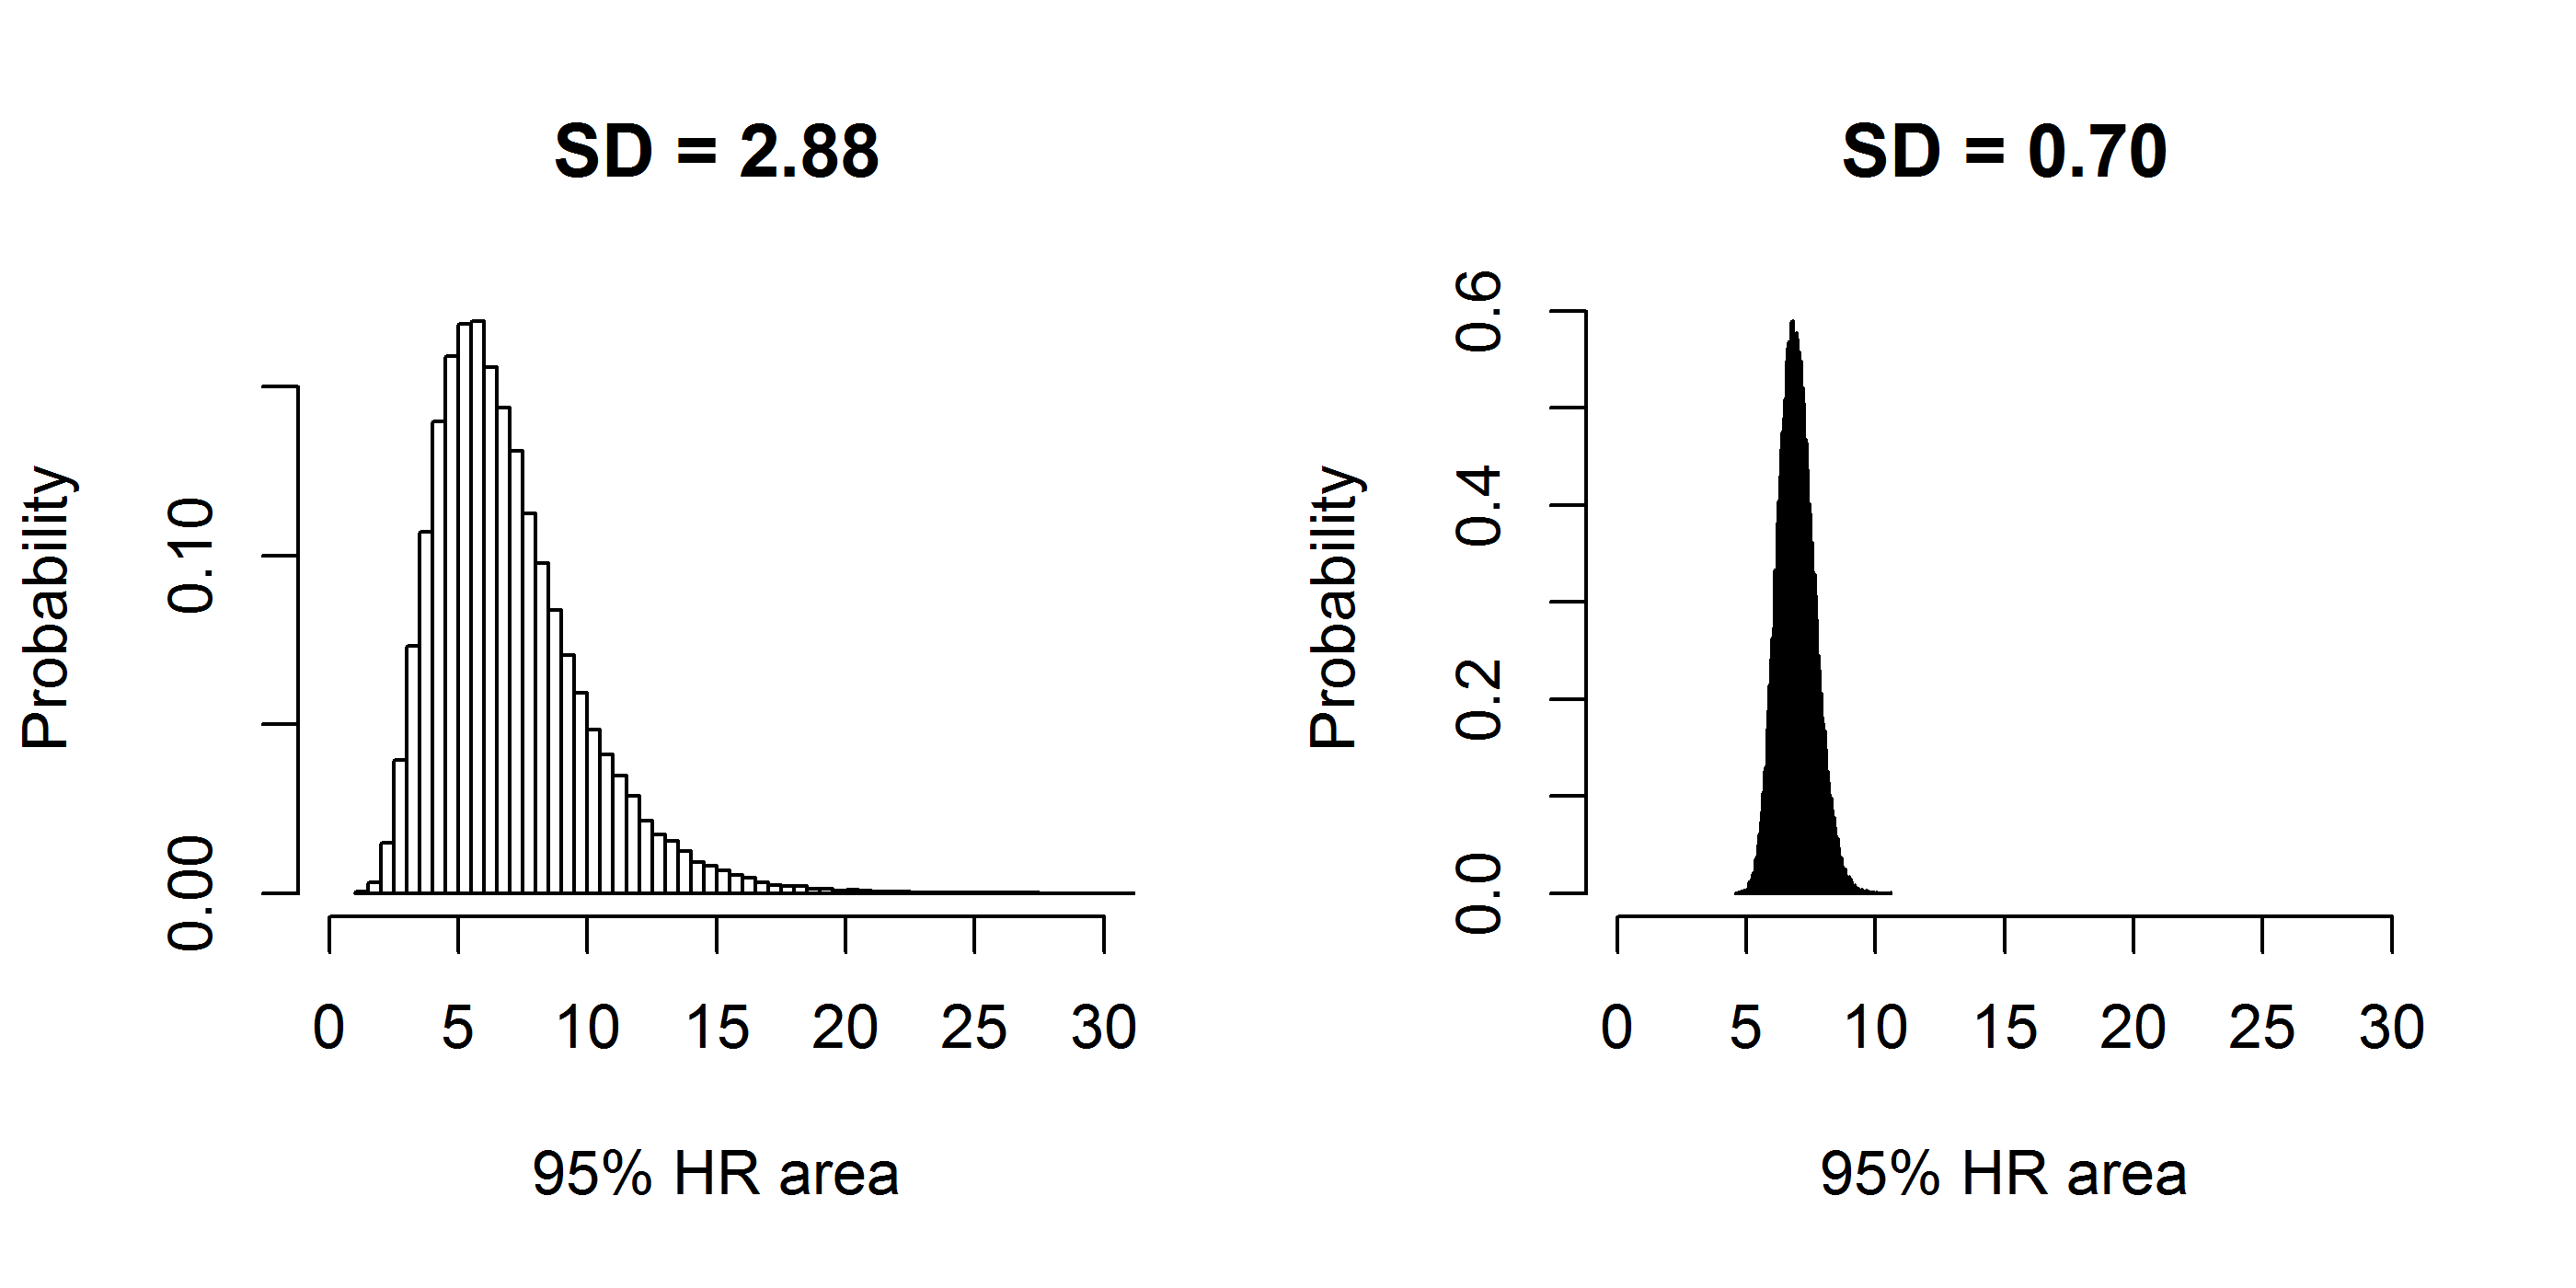
\includegraphics[height=2.5in,width=5in]{Ch8-Covariates/figs/area_heterogeneity.png}
\end{center}
\caption{
Population distribution of home range area for a model in which
$\log(\sigma^{2})$ has a normal distribution with mean $\mu_{hra}$ and
variance $\tau^{2}_{hra}$. The parameters were chosen to yield a
constant expected value of about 6.9 units of area, but to produce two
different levels of heterogeneity: A population standard deviation of
2.88 units (left panel) and 0.70 units (right panel). 
}
\label{covariates.fig.one}
\end{figure}



\section{Likelihood analysis in \secr}
\label{likelihood.secr}

Previously, in Chapt. \ref{chapt.mle}, we introduced the {\bf R}
package \secr~ and described the likelihood based inference approach taken
by that package (see Sec. \ref{mle.sec.secrguts}).  Here we discuss how
to implement some standard covariate models in \secr~ and provide an
example of model selection using AIC.   As we saw in
Chapt. \ref{chapt.mle}, \secr~ uses the standard \R~ model
specification syntax, defining the dependent and independent
variable relationship using tildes (e.g., \Verb+y ~ x+).  Thus, in
\secr~ we might have \verb+g0 ~ behavior+ or
\verb+sigma ~ time+; when left unspecified or set to 1 (e.g.,
\verb+g0 ~ 1+), this will default to a model with no covariates (i.e.,
constant parameter values).  A number of default model formulas for
the baseline and scale parameter of the encounter probability model
are available in \mbox{\tt secr}.
Additionally, \secr~ allows us to specify
covariates on density (we cover this in
Chapt. \ref{chapt.state-space}), which are set for
example as \verb+D ~ habitat+.

To demonstrate
 models with various types of covariates using \secr, we
continue using the Fort Drum black bear data. 
We include in the \scrbook package a function called {\tt secr.bear}
that will format the data (see Chapt. \ref{chapt.mle} for the \secr
data format) and then fit and compare 8 models (details shown in Panel
\ref{covariates.panel.secrfn} ).  We have described all of these
models in the previous sections, so we only briefly comment here on
how to fit certain models in \secr and compare them using AIC, and
give a few helpful notes.
% Below, 
% we have a few subsections on the sex-specific effects, heterogeneity,
% and AIC which describe in more detail how we fit these models within
% \secr.

\subsection{Notes for fitting standard models}

In the \secr package, the encounter probability model is called the
``detection function'' and it is specified 
by changing the ``\mbox{\tt detectfn}'' option (an integer code)
within the \mbox{\tt secr.fit} command.  Table
\ref{covariates.tab.detmodels} shows the possible encounter
probability models 
that \mbox{\tt secr} allows; the default is that based on the kernel
of a bivariate normal probability distribution function
(hence we call this the Gaussian model, but it is referred to as
``half-normal'' 
in \mbox{\tt secr}) and the
(negative) exponential is \mbox{\tt detectfn = 2}.  See model 2 in 
Panel \ref{covariates.panel.secrfn} for how to fit the exponential 
model to the Fort Drum bear dataset. 

The \mbox{\tt secr} package easily fits a range of SCR equivalents of standard capture-recapture models.
The package has pre-defined versions of the classic
model $M_{t}$ where each
occasion has its own encounter
 probability, as well as a linear
trend in baseline encounter probability 
over occasions (in a spatial modeling framework $\sigma$ could also be
an occasion specific parameter, but having encounter probability 
 change with time seems like the more common case). For the classical
time-effects type of model with $K$ distinct parameters \secr~ uses 't' to denote
this in the model specification formula (see model 3 in 
panel \ref{covariates.panel.secrfn}); whereas, for a linear
trend over occasions \secr~ uses 'T'.

The global trap response model (what we called model $M_{B}$), 
or a local trap-specific behavioral response (model $M_{b}$)
can be fitted in \mbox{\tt secr} using formulae with
 ``b'' for the global response model and
 ``bk'' for the local trap response model
(see models 4 and 5 in 
Panel \ref{covariates.panel.secrfn}; note that to fit the trap specific behavioral response model you need version 2.3.1 or newer of \secr).

\begin{panel}[htp]
\centering
\rule[0.1in]{\textwidth}{.03in}
{\small
\begin{verbatim}
1. null model with a bivariate normal encounter probability  model
bear_0=secr.fit(bear.cap, model=list(D ~ 1, g0 ~ 1, sigma ~ 1))

2. null model with an exponential encounter probability model
bear_0exp=secr.fit(bear.cap, model=list(D ~ 1, g0 ~ 1, sigma ~ 1),
          detectfn=2)

3. model with fixed time effects
bear_t=secr.fit(bear.cap, model=list(D ~ 1, g0 ~ t, sigma ~ 1))

4. global behavioral model
bear_B=secr.fit(bear.cap, model=list(D ~ 1, g0 ~ b, sigma ~ 1))

5. trap specific behavioral response
bear_b=secr.fit(bear.cap, model=list(D ~ 1, g0 ~ bk, sigma ~ 1))

6. global behavior model with fixed time effects
bear_bt=secr.fit(bear.cap, model=list(D ~ 1, g0 ~ b+t, sigma ~ 1))

7. sex-specific model
bear_sex=secr.fit(bear.cap, model=list(D ~ session, g0 ~ session, 
         sigma ~ session))

8. heterogeniety model
bear_h2=secr.fit(bear.cap, model=list(D ~ 1, g0 ~ h2, sigma ~ h2))
\end{verbatim}
}

\rule[-0.1in]{\textwidth}{.03in}
\caption{
Models called from \mbox{\tt secr.bear} function. All models use \mbox{\tt buffer = 20000}}
\label{covariates.panel.secrfn}
\end{panel}


\subsection{Sex Effects}
\label{covariates.secr.sex}

Incorporating sex effects into
models with \secr~ can be done a few different ways, but there are not
pre-defined models for this.  A limitation of fitting models with sex
effects in \mbox{\tt secr} is that it does not accommodate missing
values of the sex variable. Thus, in all cases,
individuals that are of unknown sex must be removed from the dataset
(recall that in a Bayesian framework we can keep these individuals in
the data set by specifying a distribution for the individual covariate
``sex'').
In \mbox{\tt secr}, the easiest way to include sex effects is 
to code sex as a  ``session'' variable using the multi-session models
(see Sec. \ref{mle.sec.multisession} for a description
of the multi-session models), providing two sessions, one representing
males and one for females (see model 7 in Panel
\ref{covariates.panel.secrfn}).  This method provides two separate
density estimates, which can then be combined into a total density.

\begin{comment}
There are a few ways that one could
specify the model with sex-specific parameters  in \mbox{\tt secr} (M. Efford, pers. comm).  One way is that we could
list sex as a categorical individual covariate in a Huggins-Alho type
model \citep{borchers_efford:2008}.
 A similar approach is to treat males and 
females as groups (in \secr~ denoted by ``g''), specify the
model as $model = list(D~g, g0~g, \sigma~g)$ and list \mbox{\tt groups = 'sex'}
where we have specified sex as a 2-level individual covariate.    The \secr~ manual suggests that for many purposes,
using the `session' implementation is equivalent to the 'groups' with the caveat that the latter is often simpler
to implement partially due to the fact that multi-session models require the detector array and mask to be 
specified separately for each session.
\end{comment}


\subsection{Individual heterogeneity}
\label{covariates.sec.secrH2}

To incorporate heterogeneity, \secr fits a set of 
finite mixture models \citep{norris_pollock:1996,
  pledger:2000}. These are expensive in terms of parameters but 
they have been widely adopted because they are easy to analyze using
likelihood methods, as the marginal distribution of the data is just a
sum of a small number of components.
Using \secr,  individual heterogeneity can be incorporated
into the encounter probability model using default models for 
 either a 2- or 3-component finite
mixture model 
using the  ``\mbox{\tt h2}'' or
``\mbox{\tt h3}'' model terms.
 The 2-part mixture is shown in model 8 of panel
\ref{covariates.panel.secrfn} and the 3-part mixture can easily be fit by
substituting \mbox{\tt h3} for \mbox{\tt h2}.  
The finite-mixture model 
can be fit in \jags~ or \bugs, but we only showed
the SCR + Mh logit-normal mixture in the version above (see
Sec. \ref{covariates.sec.heterogeneity}).



\subsection{Model selection in \secr~ with AIC}

One practical advantage to using the \secr~ package, or likelihood
inference in general, is the convenience of automatic model selection
using AIC \citep{burnham_anderson:2002}. The \mbox{\tt secr} package
has a number of convenient functions for computing AIC and producing
model selection tables, or doing model-averaging (as described in
 Chapt. \ref{chapt.gof}).
Running the function {\tt secr.bear}, which calls all of the models we
have described, will return, in addition to all model results, 
an AIC table with all of the summarized results including the AIC values,
delta AIC, and model weights (see Table \ref{covariates.tab.secrAIC}
or reproduce results in {\tt R} using {\tt out<- secr.bear(); out\$AIC.tab}). 


It is important to note that AIC is not comparable 
between a multi-session model and a model that is not a multi-session model.
Therefore, to compare the sex-specific model (which uses ``sessions") with all the other models
including the null, time, and behavioral models, we coded the dataset as a 
multi-session design when first loading it to \secr.  This results in 
all the model outputs listing separate parameter estimates for each session, even the null model
with no covariates; however, the estimates are the same for both ``sessions''
in all but the sex specific model. 


\begin{table}[ht]
\centering
\caption{Log-likelihood, AIC, deltaAIC and AIC weight for several models run in secr for the Fort Drum black bear data set.}
\begin{tabular}{crrrrr}
\hline \hline
model     &  logLik   &   AIC    &   AICc   & dAICc  & AICwt \\ \hline
bear.b    & -641.7215 & 1291.443 & 1292.395 & 0.000  &  1 \\
bear.h2   & -653.8382 & 1319.676 & 1321.776 & 29.381 &  0 \\
bear.0exp & -663.9152 & 1333.830 & 1334.389 & 41.994 &  0 \\
bear.B    & -677.6175 & 1363.235 & 1364.187 & 71.792 &  0 \\
bear.bt   & -668.3044 & 1358.609 & 1366.152 & 73.757 &  0 \\
bear.sex  & -677.7151 & 1367.430 & 1369.530 & 77.135 &  0 \\
bear.t    & -674.4134 & 1368.827 & 1374.938 & 82.543 &  0 \\
bear.0    & -686.2455 & 1378.491 & 1379.049 & 86.654 &  0 \\ \hline
\end{tabular}
\label{covariates.tab.secrAIC}
\end{table}


The results from this AIC analysis are straightforward to interpret; the model
with a local trap response of encounter probability, ``bk'', has a model weight of 1 and thus, according to AIC, 100\% support.
The 2-part finite mixture model for $g_0$ and $\sigma$ has the second lowest
AIC, but considering the large dAICc compared to the local trap response model we would probably not consider it any further.  
% Using the AIC provides a fast and convenient mechanism for
% conducting model comparisons. 


\section{Summary and Outlook}

There are endless covariates and encounter probability models that can
be defined and our goal in this chapter was to introduce basic types
of covariate models and demonstrate how to implement them in {\bf
  BUGS} and \mbox{\tt secr}.  Essentially, SCR's are GLMMs and
therefore we develop covariate models in much the same way, using a
suitable transformation (link function) of the parameter(s). In SCR
models, we typically have 2 parameters of the encounter probability
model for which we might specify covariate models -- the baseline
encounter probability (or rate) parameter, and a scale parameter that
is related in many cases to the home range size of the species.  A few
examples of different covariate models are given in Table
\ref{covariates.tab.covclass}.  We can also consider covariates by
their classification as fixed, partially observed, or unobserved (see
Table \ref{covariates.tab.covobs}). This classification of covariate
types can be important because the MLE and Bayesian approaches to
dealing with partially and unobserved covariates is often different.
This was seen above in how the covariate \mbox{\tt Sex} was handled in
the two frameworks.

\begin{table}[ht]
\centering
\caption{Examples of different covariate classifications.}
\begin{tabular}{cr}
\hline \hline
Covariate class & Examples \\
\hline 
Fixed & baited, weather, habitat\\
Partially observed & sex, age, \\
Unobserved &  home range size, ind. effects  \\ \hline
\end{tabular}
\label{covariates.tab.covobs}
\end{table}

While the move to spatially explicit models in capture-recapture
studies has largely rendered the basic CR models
\citep{otis_etal:1978} obsolete, we continue to find this
classification useful for categorizing the {\it spatial} extensions of
these standard CR models.  The extended models include the standard
$M_0$, $M_t$, $M_b$, and $M_h$, but also new models that allow for
trap-specific information such as "baited/not-baited" or "on/off
road".  In addition, in Chapts. \ref{chapt.ecoldist}, \ref{chapt.rsf}
and \ref{chapt.state-space}, we explore additional models for
explaining variation in encounter probability and density based on
spatial covariates that describe variation in landscape or habitat
conditions.

%Researchers are often concerned with describing the factors or
%covariates that influence variation in detection or encounter
%probability, particularly as this can directly influence other
%parameters in the model such as density.  These covariates have
%various levels -- specific to individual, trap, sampling occasion and
%can be fully or partially observed as well as completely latent.  In
%SCR models, these more complex covariate models are fairly easy to
%fit, though one should take caution not to over parameterize the
%models particularly when a study yields a sparse data set.


\begin{comment}
Different detection models: We can make up detection models {\it all fucking
day}, to no end, with no point, and with no biological justification for
any single model. To us this would be bad practice and so we think it is
perfectly fine to pick a model ahead of time and stick with it.

we note that underlying these different models is basically something
to do with the 2nd moment structure of some correlated spatial process...
i.e., correlation functions (Higdon et al. 1998; etc...) and , insofar
as choosing detection functions is like choosing a correlation function,
it probably wont have much affect on inferences.
\end{comment}


\begin{comment}
XXXX Andy sez: probably not -- we can stop here at a basic
description of the models XXXX

XXX Andy, do you still think this is necessary? XXX
It is interesting to consider alternative distributions for $\alpha_{1,i}$, here we 
use a Normal prior which might result in a negative value for $\alpha_{1,i}$ which is
not expected but also not entirely nonsensical.  We could also use the the Inverse-Gamma
distribution, but it is not conjugate in the present context and so
there is no compelling reason to do that.  Also important to note is that if A[i] 
is the home range area of individual $i$, and we have related area to $\sigma$ through a specified
function, then we can move back and forth between distributions for
A[i], $\sigma_i$, and $\alpha_{1,i}$.


{\bf Approximation: }
Note that ``SCR + Mh'' might be a good approximation to ``SCR + Ah''.  If we write $\alpha_{1,i} =
\alpha_{1} + \eta_{i}$ then
we can take the expectation over  $\alpha_{i}$ to arrive at
\[
\mbox{logit}(p0) = \alpha_0 
p_{ijk} = p0 \exp(- \alpha_{1}*||{\bf s}_{i}-{\bf x}_{j}||^2) +  \eta_{i}*||{\bf s}_{i}-{\bf x}_{j}||^2)
\]

Which has this additive individual effect that varies also by trap. It might be that approximating
this by SCR+Mh is better than nothing and it could also be viewed as suggesting an 
over-dispersed count model for encounter frequencies.

XXXXXXXXXXXXXXXXX above commented out 

\end{comment}